\documentclass[12pt]{article}

\usepackage{graphicx}
\usepackage{amsmath}
\usepackage{amssymb}
\usepackage{natbib}
\usepackage{amsfonts}
\usepackage{multicol}
\usepackage{float}
\usepackage{oldgerm}
\usepackage{bm}
\usepackage{mathtools}
\usepackage{wrapfig}
\usepackage{fancyhdr}
\usepackage[export]{adjustbox}
\usepackage{xcolor}

\pagestyle{empty}

\newcommand{\avec}{{\mathbf A}}
\newcommand{\bvec}{\mathbf B}
\newcommand{\dvec}{\mathbf D}
\newcommand{\evec}{\mathbf E}
\newcommand{\fvec}{\mathbf F}
\newcommand{\jvec}{\mathbf J}
\newcommand{\kvec}{{\mathbf {k}}}
\newcommand{\mvec}{{\mathbf {M}}}
\newcommand{\nbold}{{\mathbf n}}
\newcommand{\vvec}{\mathbf{v}}
\newcommand{\xvec}{{\mathbf x}}
\newcommand{\yvec}{{\mathbf y}}
\newcommand{\zvec}{{\mathbf z}}
\newcommand{\nablav}{\boldsymbol{\nabla}}
\newcommand{\phivec}{\boldsymbol{\phi}}
\newcommand{\epvec}{\boldsymbol{\epsilon}}
\newcommand{\ezero}{\epsilon_{0}}
\newcommand{\mzero}{\mu_{0}}
\newcommand{\unitx}{\mathbf{\hat{x}}}
\newcommand{\unity}{\mathbf{\hat{y}}}
\newcommand{\unitz}{\mathbf{\hat{z}}}
\newcommand{\mubold}{\boldsymbol{\mu}}
\newcommand{\uniti}{\hat{\boldsymbol{\imath}}}
\newcommand{\unitj}{\hat{\boldsymbol{\jmath}}}
\newcommand{\unitk}{\hat{\boldsymbol{\mathit{k}}}}
\newcommand{\unitn}{\hat{\mathbf n}}
\newcommand{\unitr}{\hat{\mathbf r}}
\newcommand{\unitphi}{\hat{\boldsymbol{\phi}}}
\newcommand{\unittheta}{\hat{\boldsymbol{\theta}}}

\newcommand{\bit}{\begin{itemize}}
\newcommand{\eit}{\end{itemize}}

\setlength{\headsep}{0.5cm}
\setlength{\oddsidemargin}{-0.5cm}
\setlength{\textwidth}{16.5cm}
\setlength{\textheight}{24cm}
\voffset = -2cm

\pagestyle{fancy}
\fancyhf{}
\rfoot{
\includegraphics[width=1.0in]{cnm.png}}
\lfoot{In Class Problems 1}
\begin{document}

%{\bf \underline{STUDENT NAME}:} 
%\vspace{1cm}

\begin{center}
%\date{10/02/18-10/09/18}
\hfil
{\large\bf {ENGR 2910-101: Circuit Analysis}}
\hfill Instructor: Brian Rashap\\
In Class 1: 01/11/23 \\
\hrulefill\\
\end{center}

%{\em Show all your working to ensure you obtain full points. Partial
%  credit will be given for correct algebraic steps if you fail to
%  obtain the correct final answer.}\\

%\newpage


\noindent
{\bf Question 1} %P1.7

\begin{figure}[h!]
  \centering 
  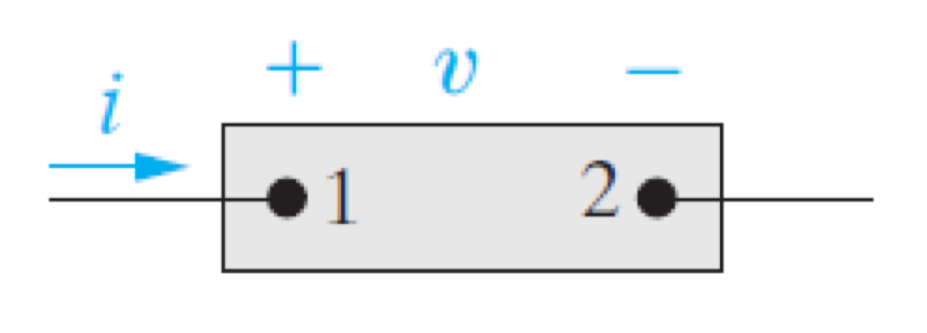
\includegraphics[clip,width=0.25\textwidth]{Fig1-5.eps}
\end{figure}

\noindent
The current entering the left terminal of this element is

\[
i = 40 \cos{(4000 t)} A
\]

\noindent
Assume the charge at the terminal is zero at the instant the current is passing through its maximum value. Find the expression for $q(t)$.

\vspace{0.3in}
\noindent
{\bf Question 2} %P1.8

\noindent
How much energy is imparted on an electron as it flows through a 6 volt battery from the positive to the negative terminal? Express your answer in attojoules ($10^{-18}$J).



\vspace{0.3in}
\noindent
{\bf Question 3}  %P1-11

\begin{figure}[h!]
  \centering 
  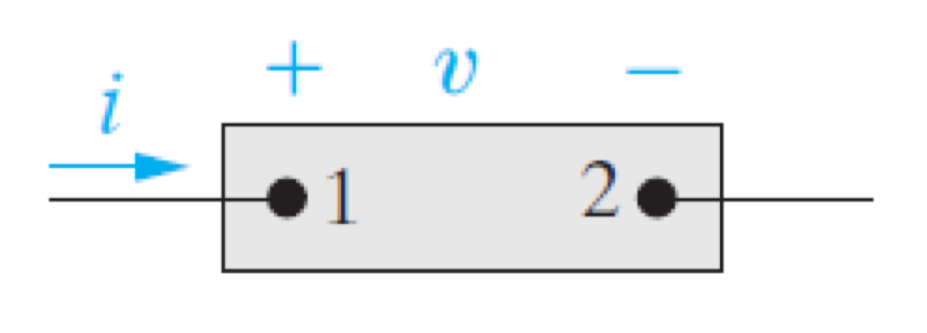
\includegraphics[clip,width=0.25\textwidth]{Fig1-5.eps}
\end{figure}

\noindent
The current at the terminals of the element is

\[
i = 40 t e^{-500 t} A \text{, for } t \geq 0 
\]

\noindent
assume $i = 0$, $t < 0$. 

\bit

\item[(a)]

Find the expression for the charge accumulating at the left electrode.

\item[(b)]

Find the charge that has accumulated at $t = 1 ms$.

\eit

\end{document}
